\section{Systemarkitektur}
Med udgangspunkt i usecasene er systemets funktionalitet forsøgt brudt ned i mindre logiske blokke. Disse skal dække over betjening af systemet, detektering af vinflaske og åbningen af denne. På baggrund af disse krav er BDD'et på figur \ref{BDD_WinePrep} udarbejdet.

\begin{figure}[H]
	\centerline{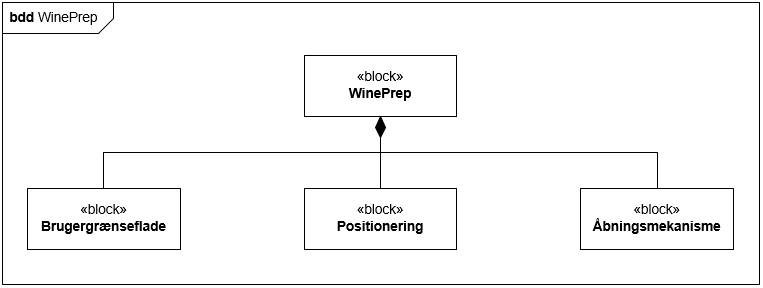
\includegraphics[scale=0.33]{tex/Arkitektur/Diagrammer/BDD_WinePrep}}
	\caption{BDD over WinePrep}
	\label{BDD_WinePrep}
\end{figure}

\noindent\textbf{Brugergrænsefladen} betjenes af bruger og initierer usecasene som beskrevet i Krav (indsæt reference hertil).
\\
\\
\textbf{Positionering} finder vinflaskens position og flytter \textbf{Åbningsmekanismen}, så den er klar til at åbne vinflasken.
\\
\\
\textbf{Åbningsmekanismen} fjerner proppen fra flasken og dispenserer denne.
\\
\\
For at forstå den interne funktionalitet og kompleksitet i blokkene \textbf{Positionering} og \textbf{Åbningsmekanisme} er disse brudt yderligere ned.

\subsubsection{Positionering}
I forhold til den specificerede afgrænsning\footnote{Se kapitlet Afgrænsning} for projektet, kræves det, at \textbf{Positionering} skal operere på tre rumlige akser: to horizontalt vinkelrette (x og y) og én vertikal (z). Derudfra kan flaskens koordinater bestemmes. Da flaskens position er statisk, forløber detekteringen sig i bevægelse langs dennes akser. \textbf{Positionering} kan dermed opdeles i to moduler: ét modul tager sig af detektering af flasken, mens det andet tager sig af bevægelsen langs akserne.

\subsubsection{Åbningsmekanisme}
Det at åbne en flaske kan brydes ned i to funktioner: \textbf{iskruning} i flaskens prop, og \textbf{proptrækning} af proppen. Derfor kan \textbf{Åbningsmekanismen} opdeles i to moduler, som tager sig af disse funktioner.

\subsection{Allokering}
De blokke, der er opstillet på figur \ref{BDD_WinePrep}, allokeres på en række fysiske blokke, som vist på figur \ref{Allokering_WinePrep}.

\begin{figure}[H]
	\centerline{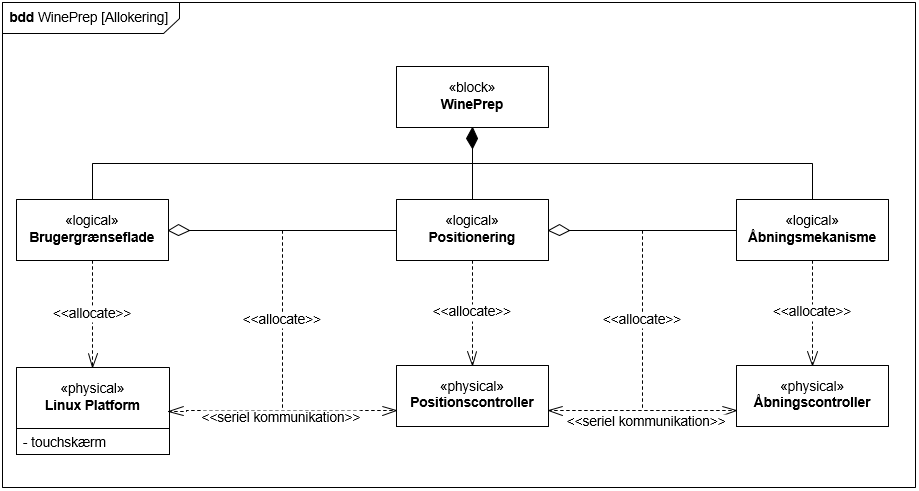
\includegraphics[scale=0.33]{tex/Arkitektur/Diagrammer/Allokering_WinePrep_to_MC}}
	\caption{Allokeringsdiagram over WinePrep}
	\label{Allokering_WinePrep}
\end{figure}

\noindent\textbf{Positionering} og \textbf{Åbningsmekanisme} er allokeret på hver deres microcontroller, som i dette projekt er besluttet til begge at være PSoC 5LP. \textbf{Brugergrænsefladen} er allokeret på en Linux-platform, som er DevKit8000.
\\
\\
\noindent Figur \ref{Allokering_WinePrep} viser ydermere allokeringen af det interne hierarki blandt blokkene. \textbf{Brugergrænsefladen} bruger \textbf{Positionering} vha. en seriel kommunikationsform. Det samme gør sig gældende mellem \textbf{Positionering} og \textbf{Åbningsmekanismen}.